\documentclass{article}
\usepackage{graphics}
\usepackage{epsfig}
\usepackage{hhline}

% define some macros:
\newcommand{\munged}{{\tt munged}}
\newcommand{\srun}{{\tt srun}}
\newcommand{\scancel}{{\tt scancel}}
\newcommand{\squeue}{{\tt squeue}}
\newcommand{\scontrol}{{\tt scontrol}}
\newcommand{\sinfo}{{\tt sinfo}}
\newcommand{\slurmctld}{{\tt slurmctld}}
\newcommand{\slurmd}{{\tt slurmd}}

\title{SLURM: Simple Linux Utility for Resource Management\thanks{
This document was prepared as an account of work sponsored by an
agency of the United States Government.  Neither the United States
Government nor the University of California nor any of their
employees, makes any warranty, express or implied, or assumes any
legal liability or responsibility for the accuracy, completeness, or
usefulness of any information, apparatus, product, or process
disclosed, or represents that its use would not infringe privately
owned rights. Reference herein to any specific commercial product,
process, or service by trade name, trademark, manufacturer, or
otherwise, does not necessarily constitute or imply its endorsement,
recommendation, or favoring by the United States Government or the
University of California.  The views and opinions of authors expressed
herein do not necessarily state or reflect those of the United States
Government or the University of California, and shall not be used for
advertising or product endorsement purposes.
This work was performed under the auspices of the U. S. Department of
Energy by the University of California, Lawrence Livermore National
Laboratory under Contract No. W-7405-Eng-48. Document UCRL-TBD.}}

\author{Morris A. Jette \and Andy B. Yoo \and Mark Grondona}

% We cheat here to easily get the desired allignment 
%\date{\{jette1,mgrondona\}@llnl.gov}
\date{Lawrence Livermore National Laboratory\\
Livermore, CA 94551\\
\{jette1,yoo2,mgrondona\}@llnl.gov}

\begin{document}

\maketitle

\begin{abstract}
Simple Linux Utility for Resource Management (SLURM) is an open source,
fault-tolerant, and highly scalable cluster management and job 
scheduling system for Linux clusters of thousands of nodes.  Components 
include machine status, partition management, job management, scheduling 
and stream copy modules.  This paper presents a overview of the SLURM architecture and functionality with an emphasis on scheduling.
\end{abstract}

\section{Overview}

SLURM\footnote{A tip of the hat to Matt Groening and creators of {\em Futurama},
where Slurm is the most popular carbonated beverage in the universe.} 
(Simple Linux Utility for Resource Management) is a resource management 
system suitable for use on Linux clusters, large and small.  After 
surveying\cite{Jette2002} resource managers available for Linux and finding 
none that were simple, highly scalable, and portable to different cluster 
architectures and interconnects, the authors set out to design a new system.

The result is a resource management system with the following general
characteristics:

\begin{itemize}
\item {\em Simplicity}: SLURM is simple enough to allow motivated end users
to understand its source code and add functionality.  The authors will 
avoid the temptation to add features unless they are of general appeal. 

\item {\em Open Source}: SLURM is available to everyone and will remain free. 
Its source code is distributed under the GNU General Public 
License\cite{GPL2002}.

\item {\em Portability}: SLURM is written in the C language, with a GNU 
{\em autoconf} configuration engine.  
While initially written for Linux, other UNIX-like operating systems 
should be easy porting targets.
SLURM also supports a general purpose {\em plugin} mechanism, which 
permits a variety of different infrastructures to be easily supported. 
The SLURM configuration file specifies which set of plugin modules 
should be used. 

\item {\em Interconnect independence}: SLURM supports UDP/IP based
communication as well as the Quadrics Elan3 and Myrinet interconnects.  
Adding support for other interconnects is straightforward and utilizes 
the plugin mechanism described above.

\item {\em Scalability}: SLURM is designed for scalability to clusters of
thousands of nodes. The SLURM controller for a cluster with 1000 nodes 
occupies on the order of 2 MB of memory and excellent performance has 
been demonstrated. 
Jobs may specify their resource requirements in a variety of ways 
including requirements options and ranges, potentially permitting 
faster initiation than otherwise possible.

\item {\em Fault tolerance}: SLURM can handle a variety of failure modes
without terminating workloads, including crashes of the node running 
the SLURM controller. 
User jobs may be configured to continue execution despite the failure 
of one or more nodes on which they are executing. 
The user command controlling a job, {\tt srun}, may detach and reattach 
from the parallel tasks at any time. 
Nodes allocated to a job are available for reuse as soon as the job(s) 
allocated to that node terminate. 
If some nodes fail to complete job termination 
in a timely fashion due to hardware of software problems, only the 
scheduling of those tardy nodes will be effected.

\item {\em Secure}: SLURM employs crypto technology to authenticate 
users to services and services to each other with a variety of options 
available through the plugin mechanism.  
SLURM does not assume that its networks are physically secure, 
but does assume that the entire cluster is within a single 
administrative domain with a common user base across the 
entire cluster.

\item {\em System administrator friendly}: SLURM is configured a 
simple configuration file and minimizes distributed state.  
Its configuration may be changed at any time without impacting running jobs. 
Heterogeneous nodes within a cluster may be easily managed.
SLURM interfaces are usable by scripts and its behavior is highly 
deterministic.

\end{itemize}

\subsection{What is SLURM?}

As a cluster resource manager, SLURM has three key functions.  First,
it allocates exclusive and/or non-exclusive access to resources 
(compute nodes) to users for 
some duration of time so they can perform work.  Second, it provides 
a framework for starting, executing, and monitoring work (normally a 
parallel job) on the set of allocated nodes.  Finally, it arbitrates 
conflicting requests for resources by managing a queue of pending work.

Users interact with SLURM through four command line utilities: 
\srun\ for submitting a job for execution and optionally controlling it
interactively, 
\scancel\ for early termination of a pending or running job, 
\squeue\ for monitoring job queues, and 
\sinfo\ for monitoring partition and overall system state.
System administrators perform privileged operations through an additional
command line utility: {\tt scontrol}.

The central controller daemon, {\tt slurmctld}, maintains the global state 
and directs operations.
Compute nodes simply run a \slurmd\ daemon (similar to a remote shell 
daemon) to export control to SLURM.  

SLURM is not a sophisticated batch system.  
In fact, it was expressly designed to provide high-performance 
parallel job management while leaving scheduling decisions to an 
external entity as will be described later. 

\subsection{Architecture}

\begin{figure}[tb]
\centerline{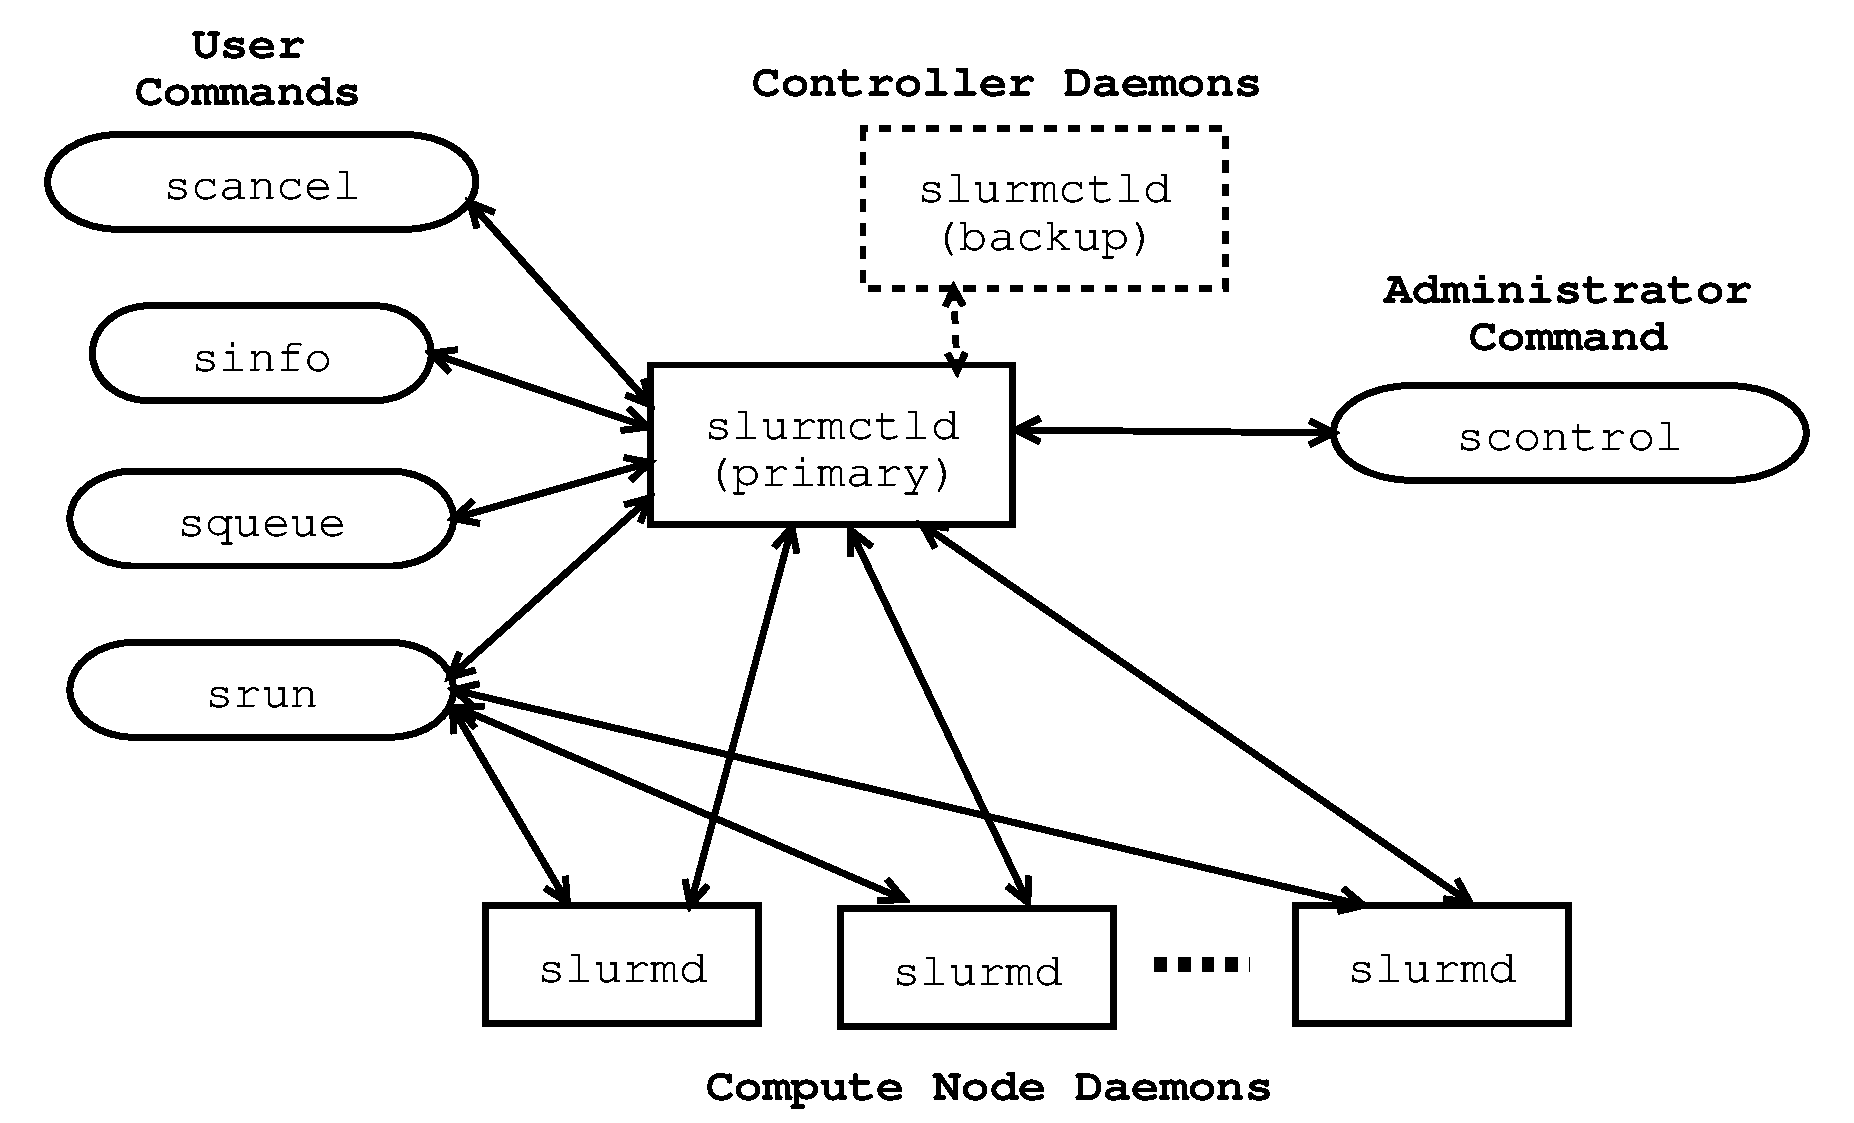
\epsfig{file=figures/arch.eps,scale=0.40}}
\caption{SLURM Architecture}
\label{arch}
\end{figure}

As depicted in Figure~\ref{arch}, SLURM consists of a \slurmd\ daemon
running on each compute node, a central \slurmctld\ daemon running on
a management node (with optional fail-over twin), and five command line
utilities: {\tt srun}, {\tt scancel}, {\tt sinfo}, {\tt squeue}, and 
{\tt scontrol}, which can run anywhere in the cluster.  

The entities managed by these SLURM daemons include {\em nodes}, the
compute resource in SLURM, {\em partitions}, which group nodes into
logical disjoint sets, {\em jobs}, or allocations of resources assigned
to a user for a specified amount of time, and {\em job steps}, which are
sets of (possibly parallel) tasks within a job.  
Each job is allocated nodes within a single partition. 
Once a job is assigned a set of nodes, the user is able to initiate
parallel work in the form of job steps in any configuration within the
allocation. For instance a single job step may be started which utilizes
all nodes allocated to the job, or several job steps may independently 
use a portion of the allocation.

\begin{figure}[tcb]
\centerline{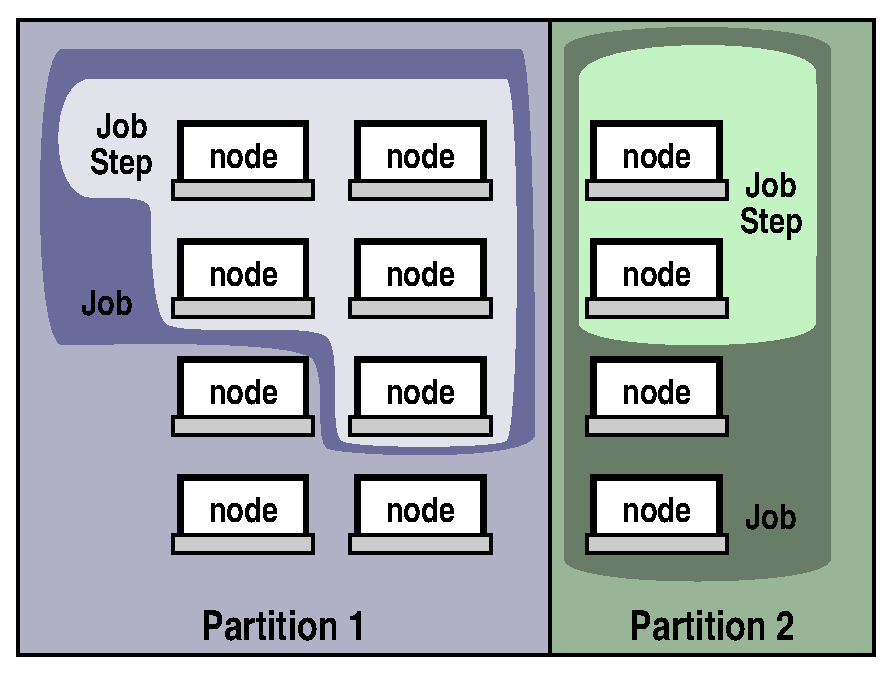
\epsfig{file=figures/entities.eps,scale=0.7}}
\caption{SLURM Entities}
\label{entities}
\end{figure}

Figure~\ref{entities} further illustrates the interrelation of these
entities as they are managed by SLURM. The diagram shows a group of
compute nodes split into two partitions. Partition 1 is running one
job, with one job step utilizing the full allocation of that job.
The job in Partition 2 has only one job step using half of the original
job allocation.
That job might initiate additional job step(s) to utilize 
the remaining nodes of its allocation.

\begin{figure}[tb]
\centerline{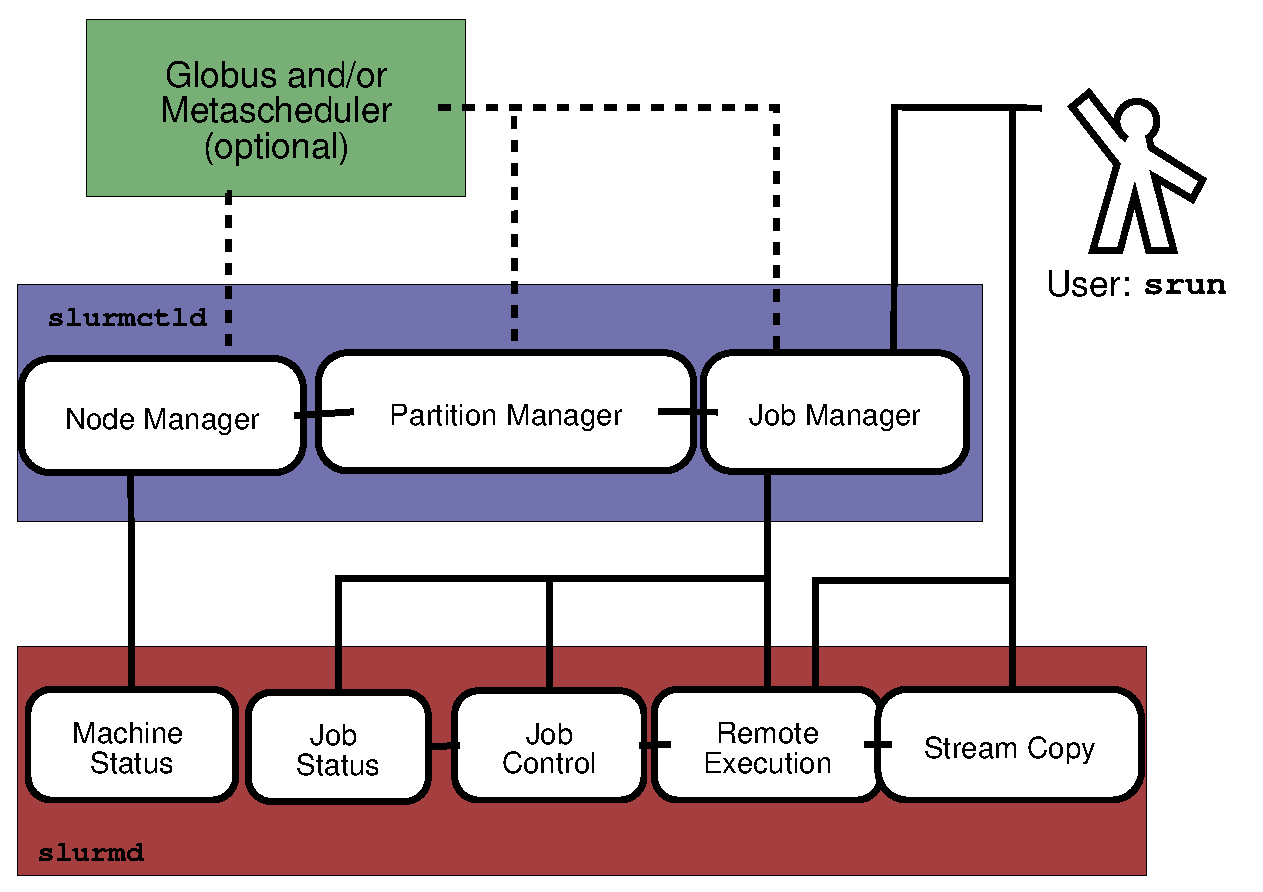
\epsfig{file=figures/slurm-arch.eps,scale=0.5}}
\caption{SLURM Architecture - Subsystems}
\label{archdetail}
\end{figure}

Figure~\ref{archdetail} exposes the subsystems that are implemented
within the \slurmd\ and \slurmctld\ daemons.  These subsystems
are explained in more detail below.

\subsubsection{Slurmd}

\slurmd\ is a multi-threaded daemon running on each compute node and 
can be compared to a remote shell daemon:  
it reads the common SLURM configuration file, 
notifies the controller that it is active, waits for work, 
executes the work, returns status,then waits for more work.  
Since it initiates jobs for other users, it must run as user {\em root}.
It also asynchronously exchanges node and job status with {\tt slurmctld}.  
The only job information it has at any given time pertains to its 
currently executing jobs.
\slurmd\ has five major components:

\begin{itemize}
\item {\em Machine and Job Status Services}:  Respond to controller 
requests for machine and job state information, and send asynchronous 
reports of some state changes (e.g. \slurmd\ startup) to the controller.

\item {\em Remote Execution}: Start, monitor, and clean up after a set
of processes (typically belonging to a parallel job) as dictated by the
\slurmctld\ daemon or an \srun\ or \scancel\ command. Starting a process may
include executing a prolog program, setting process limits, setting real
and effective user id, establishing environment variables, setting working
directory, allocating interconnect resources, setting core file paths,
initializing the Stream Copy Service, and managing
process groups. Terminating a process may include terminating all members
of a process group and executing an epilog program.

\item {\em Stream Copy Service}: Allow handling of stderr, stdout, and
stdin of remote tasks. Job input may be redirected from a file or files, a
\srun\ process, or /dev/null.  Job output may be saved into local files or
sent back to the \srun\ command. Regardless of the location of stdout/err,
all job output is locally buffered to avoid blocking local tasks.

\item {\em Job Control}: Allow asynchronous interaction with the
Remote Execution environment by propagating signals or explicit job
termination requests to any set of locally managed processes.

\end{itemize}

\subsubsection{Slurmctld}

Most SLURM state information exists in the controller, {\tt slurmctld}.
\slurmctld\ is multi-threaded with independent read and write locks 
for the various data structures to enhance scalability. 
When \slurmctld\ starts, it reads the SLURM configuration file.  
It also can read additional state information
from a checkpoint file generated by a previous execution of {\tt slurmctld}.
Full controller state information is written to 
disk periodically with incremental changes written to disk immediately
for fault tolerance.  
\slurmctld\ runs in either master or standby mode, depending on the
state of its fail-over twin, if any.
\\slurmctld\ need not execute as user {\em root}. 
In fact, it is recommended that a unique user entry be created for 
executing \slurmctld\ and that user must be identified in the SLURM 
configuration file as {\tt SlurmUser}.
\slurmctld\ has three major components:

\begin{itemize}
\item {\em Node Manager}: Monitors the state of each node in
the cluster.  It polls {\tt slurmd}'s for status periodically and
receives state change notifications from \slurmd\ daemons asynchronously.
It ensures that nodes have the prescribed configuration before being 
considered available for use.

\item {\em Partition Manager}: Groups nodes into non-overlapping sets called
{\em partitions}. Each partition can have associated with it various job
limits and access controls.  The partition manager also allocates nodes
to jobs based upon node and partition states and configurations. Requests
to initiate jobs come from the Job Manager.  \scontrol\ may be used
to administratively alter node and partition configurations.

\item {\em Job Manager}: Accepts user job requests and places pending 
jobs in a priority ordered queue. 
The Job Manager is awakened on a periodic basis and whenever there
is a change in state that might permit a job to begin running, such
as job completion, job submission, partition {\em up} transition,
node {\em up} transition, etc.  The Job Manager then makes a pass
through the priority-ordered job queue. The highest priority jobs 
for each partition are allocated resources as possible. As soon as an 
allocation failure occurs for any partition, no lower-priority jobs for 
that partition are considered for initiation. 
After completing the scheduling cycle, the Job Manager's scheduling
thread sleeps.  Once a job has been allocated resources, the Job Manager
transfers necessary state information to those nodes, permitting it 
to commence execution.  When the Job Manager detects that
all nodes associated with a job have completed their work, it initiates
clean-up and performs another scheduling cycle as described above.

\end{itemize}

\subsubsection{Command Line Utilities}

The command line utilities are the user interface to SLURM functionality.
They offer users access to remote execution and job control. They also 
permit administrators to dynamically change the system configuration. 
These commands all use SLURM APIs which are directly available for 
more sophisticated applications.

\begin{itemize}
\item {\tt scancel}: Cancel a running or a pending job or job step, 
subject to authentication and authorization. This command can also 
be used to send an arbitrary signal to all processes on all nodes 
associated with a job or job step.

\item {\tt scontrol}: Perform privileged administrative commands
such as draining a node or partition in preparation for maintenance. 
Many \scontrol\ functions can only be executed by privileged users.

\item {\tt sinfo}: Display a summary of partition and node information.
A assortment of filtering and output format options are available.

\item {\tt squeue}: Display the queue of running and waiting jobs 
and/or job steps. A wide assortment of filtering, sorting, and output 
format options are available.

\item {\tt srun}: Allocate resources, submit jobs to the SLURM queue,
and initiate parallel tasks (job steps). 
Every set of executing parallel tasks has an associated \srun\ which 
initiated it and, if the \srun\ persists, managing it. 
Jobs may be submitted for later execution (e.g. batch), in which case 
\srun\ terminates after job submission. 
Jobs may also be submitted for interactive execution, where \srun\ keeps 
running to shepherd the running job. In this case, 
\srun\ negotiates connections with remote {\tt slurmd}'s 
for job initiation and to
get stdout and stderr, forward stdin\footnote{\srun\ command
line options select the stdin handling method such as broadcast to all
tasks, or send only to task 0.}, and respond to signals from the user.
\srun\ may also be instructed to allocate a set of resources and
spawn a shell with access to those resources.

\end{itemize}

\subsubsection{Plugins}

In order to make the use of different infrastructures possible, 
SLURM uses a general purpose plugin mechanism. 
A SLURM plugin is a dynamically linked code object which is 
loaded explicitly at run time by the SLURM libraries. 
A plugin provides a customized implemenation of a well-defined
API connected to tasks such as authentication, interconnect fabric, 
task scheduling, etc.
A set of functions is defined for use by all of the different 
infrastructures of a particular variety. 
For example, the authentication plugin must define functions 
such as: 
{\em slurm\_auth\_activate} to create a credential,
{\em slurm\_auth\_verify} to verify a credential to 
approve or deny authentication, 
{\em slurm\_auth\_get\_uid} to get the user id associated with 
a specific credential, etc.
It also must define the data structure used, a plugin type, 
a plugin version number, etc. 
When a slurm daemon is initiated, it reads the configuration 
file to determine which of the available plugins should be used. 
For example {\em AuthType=auth/authd} says to use the plugin for 
authd based authentication and {\em PluginDir=/usr/local/lib} 
identifies the directory in which to find the plugin.

\subsubsection{Communications Layer}

SLURM presently uses Berkeley sockets for communications. 
However, we anticipate using the plugin mechanism to easily 
permit use of other communications layers. 
At LLNL we are using an Ethernet for SLURM communications and 
the Quadrics Elan switch exclusively for user applications. 
The SLURM configuration file permits the identification of each 
node's hostname as well as its name to be used for communications. 
In the case of a control machine known as {\em mcri} to be 
communicated with using the name {\em emcri} (say to indicate 
an ethernet communications path), this is represented in the 
configuration file as {\em ControlMachine=mcri ControlAddr=emcri}.
The name used for communication is the same as the hostname unless 
otherwise specified.

While SLURM is able to manage 1000 nodes without difficulty using 
sockets and Ethernet, we are reviewing other communication 
mechanisms which may offer improved scalability. 
One possible alternative is STORM\cite{STORM2001}. 
STORM uses the cluster interconnect and Network Interface Cards to 
provide high-speed communications including a broadcast capability. 
STORM only supports the Quadrics Elan interconnnect at present, 
but does offer the promise of improved performance and scalability. 

\subsubsection{Security}

SLURM has a simple security model: 
Any user of the cluster may submit parallel jobs to execute and cancel
his own jobs.  Any user may view SLURM configuration and state
information.  
Only privileged users may modify the SLURM configuration,
cancel any job, or perform other restricted activities.  
Privileged users in SLURM include the users {\em root} 
and {\tt SlurmUser} (as defined in the SLURM configuration file). 
If permission to modify SLURM configuration is 
required by others, set-uid programs may be used to grant specific
permissions to specific users.

We presently support three authentication mechanisms via plugins: 
{\tt authd}\cite{Authd2002}, {\tt munged} and {\tt none}. 
A plugin can easily be developed for Kerberos or authentication 
mechanisms as desired.
The \munged\ implementation is described below.
A \munged\ daemon running as user {\em root} on each node confirms the 
identify of the user making the request using the {\em getpeername} 
function and generates a credential. 
The credential contains a user id, 
group id, time-stamp, lifetime, some pseudo-random information, and 
any user supplied information. \munged\ uses a private key to 
generate a Message Authentication Code (MAC) for the credential.
\munged\ then uses a public key to symmetrically encrypt 
the credential including the MAC. 
SLURM daemons and programs transmit this encrypted 
credential with communications. The SLURM daemon receiving the message 
sends the credential to \munged\ on that node. 
\munged\ decrypts the credential using its private key, validates it 
and returns the user id and group id of the user originating the 
credential.
\munged\ prevents replay of a credential on any single node 
by recording credentials that have already been authenticated.
In SLURM's case, the user supplied information includes node 
identification information to prevent a credential from being 
used on nodes it is not destined for.

When resources are allocated to a user by the controller, a 
{\em job step credential} is generated by combining the user id, job id, 
step id, the list of resources allocated (nodes), and the credential
lifetime. This job step credential is encrypted with 
a \slurmctld\ private key. This credential 
is returned to the requesting agent ({\tt srun}) along with the
allocation response, and must be forwarded to the remote {\tt slurmd}'s 
upon job step initiation. \slurmd\ decrypts this credential with the
\slurmctld 's public key to verify that the user may access
resources on the local node. \slurmd\ also uses this job step credential 
to authenticate standard input, output, and error communication streams. 

Access to partitions may be restricted via a {\em RootOnly} flag.  
If this flag is set, job submit or allocation requests to this 
partition are only accepted if the effective user ID originating 
the request is a privileged user. 
The request from such a user may submit a job as any other user. 
This may be used, for example, to provide specific external schedulers
with exclusive access to partitions.  Individual users will not be 
permitted to directly submit jobs to such a partition, which would 
prevent the external scheduler from effectively managing it.  
Access to partitions may also be restricted to users who are 
members of specific Unix groups using a {\em AllowGroups} specification.

\section{Scheduling Infrastructure}

Scheduling parallel computers is a very complex matter.  
Several good public domain schedulers exist with the most 
popular being the Maui Scheduler\cite{Jackson2001,Maui2002}. 
The scheduler used at our site, DPCS\cite{DPCS2002}, is quite 
sophisticated and has over 150,000 lines of code. 
We felt no need to address scheduling issues within SLURM, but 
have instead developed a resource manager with a rich set of 
application programming interfaces (APIs) and the flexibility 
to satisfy the needs of others working on scheduling issues.  
SLURM's default scheduler implements First-In First-Out (FIFO). 
An external entity can establish a job's initial priority 
through a plugin.
An external scheduler may also submit, signal, hold, reorder and 
terminate jobs via the API.

\subsection{Resource Specification}

The \srun\ command and corresponding API have a wide of resource 
specifications available. The \srun\ resource specification options 
are described below.

\subsubsection{Geometry Specification}

These options describe how many nodes and tasks are needed as
well as describing the distribution of tasks across the nodes.

\begin{itemize}
\item {\tt cpus-per-task=<number>}: 
Specifies the number of processors cpus) required for each task 
(or process) to run. 
This may be useful if the job is multithreaded and requires more 
than one cpu per task for optimal performance. 
The default is one cpu per process.

\item {\tt nodes=<number>[-<number>]}: 
Specifies the number of nodes required by this job. 
The node count may be either a specific value or a minimum and maximum 
node count separated by a hyphen. 
The partition's node limits supersede those of the job. 
If a job's node limits are completely outside of the range permitted 
for it's associated partition, the job will be left in a PENDING state. 
The default is to allocate one cpu per process, such that nodes with 
one cpu will run one task, nodes with 2 cpus will run two tasks, etc.
The distribution of processes across nodes may be controlled using 
this option along with the {\tt nproc} and {\tt cpus-per-task} options.

\item {\tt nprocs=<number>}: 
Specifies the number of processes to run. 
Specification of the number of processes per node may be achieved 
with the {\tt cpus-per-task} and {\tt nodes} options. 
The default is one process per node unless {\tt cpus-per-task} 
explicitly specifies otherwise.

\end{itemize}

\subsubsection{Constraint Specification}

These options describe what configuration requirements of the nodes 
which can be used.

\begin{itemize}

\item {\tt constraint=list}: 
Specify a list of constraints. The list of constraints is
a comma separated list of features that have been assigned to the
nodes by the slurm administrator. If no nodes have the requested
feature, then the job will be rejected.

\item {\tt contiguous=[yes|no]}: 
demand a contiguous range of nodes. The default is "yes". 

\item {\tt mem=<number>}: 
Specify a minimum amount of real memory per node (in megabytes).

\item {\tt mincpus=<number>}: 
Specify minimum number of cpus per node.

\item {\tt partition=name}: 
Specifies the partition to be used. 
There will be a default partition specified in the SLURM configuration file.

\item {\tt tmp=<number>}: 
Specify a minimum amount of temporary disk space per node (in megabytes).

\item {\tt vmem=<number>}: 
Specify a minimum amount of virtual memory per node (in megabytes).

\end{itemize}

\subsubsection{Other Resource Specification}

\begin{itemize}

\item {\tt batch}: 
Submit in "batch mode." 
srun will make a copy of the executable file (a script) and submit therequest for execution when resouces are available.
srun will terminate after the request has been submitted. 
The executable file will run on the first node allocated to the 
job and must contain srun commands to initiate parallel tasks.

\item {\tt exclude=[filename|node\_list]}: 
Request that a specific list of hosts not be included in the resources 
allocated to this job. The host list will be assumed to be a filename 
if it contains a "/"character. If some nodes are suspect, this option 
may be used to avoid using them.

\item {\tt immediate}: 
Exit if resources are not immediately available. 
By default, the request will block until resources become available.

\item {\tt nodelist=[filename|node\_list]}: 
Request a specific list of hosts. The job will contain at least
these hosts. The list may be specified as a comma-separated list of
hosts, a range of hosts (host[1-5,7,...] for example), or a filename.
The host list will be assumed to be a filename if it contains a "/"
character.

\item {\tt overcommit}: 
Overcommit resources. 
Normally the job will not be allocated more than one process per cpu. 
By specifying this option, you are explicitly allowing more than one process
per cpu. 

\item {\tt share}: 
The job can share nodes with other running jobs. This may result in faster job 
initiation and higher system utilization, but lower application performance.

\item {\tt time=<number>}: 
Establish a time limit to terminate the job after the specified number of 
minutes. If the job's time limit exceed's the partition's time limit, the 
job will be left in a PENDING state. The default value is the partition's 
time limit. When the time limit is reached, the job's processes are sent 
SIGXCPU followed by SIGKILL. The interval between signals is configurable.

\end{itemize}

All parameters may be specified using single letter abbreviations 
("-n" instead of "--nprocs=4"). 
Environment variable can also be used to specify many parameters. 
Environment variable will be set to the actual number of nodes and 
processors allocated
In the event that the node count specification is a range, the 
application could inspect the environment variables to scale the 
problem appropriately.
To request four processes with one cpu per task the command line would 
look like this: {\em srun --nprocs=4 --cpus-per-task=1 hostname}.
Note that if multiple resource specifications are provided, resources 
will be allocated so as to satisfy the all specifications. 
For example a request with the specification {\tt nodelist=dev[0-1]} 
and {\tt nodes=4} may be satisfied with nodes {\tt dev[0-3]}.

\subsection{The Maui Scheduler and SLURM}

{\em The integration of the Maui Scheduler with SLURM was 
just beginning at the time this paper was written. Full 
integration is anticipated by the time of the conference.
This section will be modified as needed based upon that 
experience.}

The Maui Scheduler is integrated with SLURM through the 
previously described plugin mechanism. 
The previously described SLURM commands are used for 
all job submissions and interactions. 
When a job is submitted to SLURM, a Maui Scheduler module 
is called to establish its initial priority. 
Another Maui Scheduler module is called at the beginning 
of each SLURM scheduling cycle. 
Maui can use this opportunity to change priorities of 
pending jobs or take other actions.

\subsection{DPCS and SLURM}

DPCS is a meta-batch system designed for use within a single 
administrative domain (all computers have a common user ID 
space and exist behind a firewall). 
DPCS presents users with a uniform set of commands for a wide 
variety of computers and underlying resource managers (e.g. 
LoadLeveler on IBM SP systems, SLURM on Linux clusters, NQS, 
etc.). 
It was developed in 1991 and has been in production use since 
1992. 
While Globus\cite{Globus2002} has the ability to span administrative 
domains, both systems could interface with SLURM in a similar fashion.

Users submit jobs directly to DPCS.
The job consists of a script and an assortment of constraints. 
Unless specified by constraints, the script can execute on 
a variety of different computers with various architectures 
and resource managers. 
DPCS monitors the state of these computers and performs backfill 
scheduling across the computers with jobs under its management. 
When DPCS decides that resources are available to immediately 
initiate some job of its choice, it takes the following 
actions:
\begin{itemize}
\item Transfers the job script and assorted state information to 
the computer upon which the job is to execute.

\item Allocates resources for the job. 
The resource allocation is performed as user {\em root} and SLURM 
is configured to restrict resource allocations in the relevent 
partitions to user {\em root}.
This prevents user resource allocations to that partition
except through DPCS, which has complete control over job 
scheduling there.
The allocation request specifies the target user ID, job ID 
(to match DPCS' own numbering scheme) and specific nodes to use.

\item Spawns the job script as the desired user.
This script may contain multiple instantiations of \srun\ 
to initiate multiple job steps. 

\item Monitor the job's state and resource consumption. 
This is performed using DPCS daemons on each compute node 
recording CPU time, real memory and virtual memory consumed. 

\item Cancel the job as needed when it has reached its time limit. 
The SLURM job is initiated with an infinite time limit. 
DPCS mechanisms are used exclusively to manage job time limits. 

\end{itemize}

Much of the SLURM functionality is left unused in the DPCS 
controlled environment. 
It should be noted that DPCS is typically configured to not 
control all partitions. 
A small (debug) partition is typically configured for smaller 
jobs and users may directly use SLURM commands to access that 
partition.

\section{Results}

\begin{figure}[htb]
\centerline{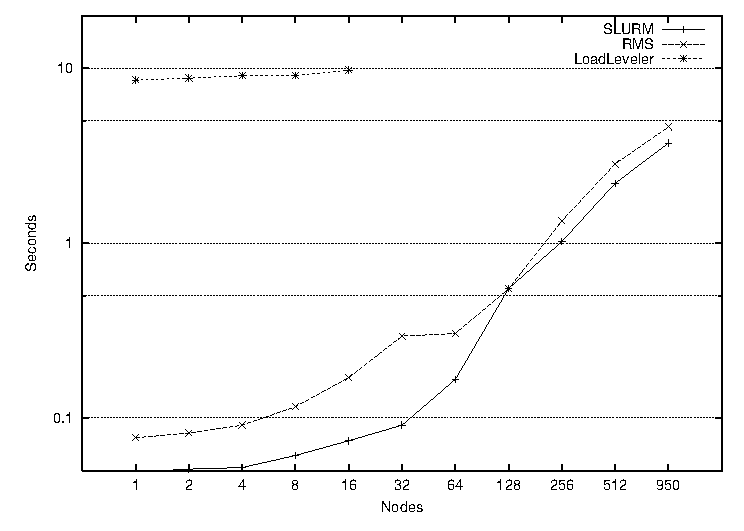
\epsfig{file=figures/times.eps}}
\caption{Time to execute /bin/hostname with various node counts}
\label{timing}
\end{figure}

We were able to perform some SLURM tests on a 1000 node cluster in 
November 2002. Some development was still underway at that time and 
tuning had not been performed. The results for executing the program 
{\em /bin/hostname} on two tasks per node and various node counts is show 
in Figure~\ref{timing}. We found SLURM performance to be comparable 
to the Quadrics Resource Management System (RMS)\cite{Quadrics2002} 
for all job sizes and about 80 times faster than IBM 
LoadLeveler\cite{LL2002} at tested job sizes.

\section{Future plans}

We expect SLURM to begin production use on LLNL Linux clusters 
starting in March 2003 and be available for distribution shortly 
thereafter. 

Looking ahead, we anticipate adding support for additional 
operating systems (IA64 and x86-64) and interconnects (InfiniBand
and the IBM Blue Gene\cite{BlueGene2002} system\footnote{Blue Gene 
has a different interconnect than any supported by SLURM and 
a 3-D topography with restrictive allocation constraints.}). 
We anticipate adding a job preempt/resume capability to 
the next release of SLURM. 
This will provide an external scheduler the infrastructure 
required to perform gang scheduling. 
We also anticipate adding a checkpoint/restart capability 
at some time in the future. 
We also plan to support changing the node count associated 
with running jobs (as needed for MPI2). 
Recording resource use by each parallel job is planned for a 
future release.

\section{Acknowledgments}

Additional programmers are responsible for the development of 
SLURM include: Chris Dunlap, Joey Ekstrom, Jim Garlick, Kevin Tew
and Jay Windley.

\bibliographystyle{plain}
\bibliography{project}

\end{document}
